As the climate warms and urban-wildland interfaces expand, wildfires, structural collapses, and industrial accidents are occurring with unprecedented frequency and severity \cite{erdelj2017help}. In time-critical disaster management, early and dependable detection is essential to preserve human life and contain environmental damage. Contemporary emergency monitoring relies heavily on satellite-based observation and ground sensor networks, yet both suffer from inherent operational constraints: satellites exhibit infrequent revisit intervals (5--16 days) and cloud obscuration, while ground sensor networks provide only localized point coverage with costly infrastructure requirements.

Unmanned Aerial Vehicles (UAVs) provide a transformative airborne capability, offering agile deployment, sub-meter spatial resolution, and dynamic trajectory adjustment over hazardous terrains inaccessible to human responders \cite{merino2012unmanned}. However, real-time autonomous disaster response demands more than coarse image-level classification: UAVs must perform \textbf{dense spatial object detection} to accurately localize active flame fronts, diffuse smoke plumes, and isolated survivors $(\text{xmin}, \text{ymin}, \text{xmax}, \text{ymax})$ to direct targeted water drops and search-and-rescue teams.

Single-modality airborne sensing is fundamentally brittle: RGB visual cameras fail under heavy smoke occlusion, low illumination, and glare; thermal infrared cameras suffer from low spatial resolution (typically $320\times240$ px) and generate false-positive bounding boxes triggered by solar-heated metal roofs and bare soil; and onboard acoustic sensing can be affected by UAV rotor and environmental noise~\cite{gupta2025droneaudioset}. While multimodal fusion can theoretically overcome these single-sensor failure modes, existing aerial fusion frameworks face major technical barriers: (1) high computational complexity exceeding the power and latency budgets of embedded UAV edge accelerators; (2) static, fixed-weight fusion strategies that cannot dynamically down-weight blinded or corrupted cameras; and (3) multi-task negative transfer where dense bounding box regression gradients corrupt shared classification features during end-to-end joint training \cite{baltrusaitis2019multimodal, yu2020gradient}.

\section{Background}

UAV-based disaster perception requires combining heterogeneous aerial sensor streams, such as visual RGB video, thermal infrared imagery, and acoustic signatures, into a coherent spatial and semantic representation \cite{merino2012unmanned, baltrusaitis2019multimodal}. In operational flight, sensor reliability dynamically shifts with smoke density, flight altitude, time of day, and environmental acoustics. An autonomous system must perform two complementary levels of perception: (i) \textit{global scene understanding} to categorize the overarching disaster type and evaluate overall sensor trust, and (ii) \textit{dense multi-scale object detection} to localize specific hazard objects and survivors. Combining these tasks within an integrated, failure-resilient architecture without prohibitive computational overhead is the core objective of this research.

\textbf{Data limitation that frames all results.} No public dataset used here provides synchronized RGB, thermal and audio recordings of the same UAV scene. In the assembled collection, every thermal input is a pseudo-thermal map computed from the RGB frame rather than a radiometric LWIR measurement from independent hardware, and every audio input is an ESC-50 clip assigned to visual rows by shared label rather than recorded with them. The ``multimodal'' fusion evaluated in this work is therefore fusion of RGB with an RGB-derived representation and label-matched audio. It cannot detect phenomena invisible to RGB, cannot exercise complementary sensor failures (for example, RGB dark while LWIR remains clear), and the two-sensor subsets do not validate an independent thermal fallback. Evaluation with hardware-synchronized RGB, LWIR and on-board audio remains future work.

\section{Rationale and Motivation}

When disaster detection and localization are delayed, the scale of destruction expands exponentially. For wildfire management, early bounding-box localization of emergent ignition points within the first 15--30 minutes reduces total burned area by 40--60\% and suppression costs by up to 75\%~\cite{merino2012unmanned}. In search-and-rescue (SAR) operations, locating trapped survivors within the initial 24 hours yields survival rates exceeding 90\%, whereas delays exceeding 72 hours drop survival rates below 25\%~\cite{erdelj2017help}.

Current automated aerial detection systems suffer from high false-positive rates (12--18\%), triggering costly and hazardous emergency deployments to solar reflections or dust clouds. Furthermore, naive joint training of multi-task networks (simultaneous scene classification and bounding box regression) frequently causes negative transfer, where conflicting gradient signals degrade classification accuracy by up to 45\%. These operational challenges motivate a lightweight, unified perception architecture that uses physical priors and reliability gating, with the goals of low training cost, sub-20ms inference latency, and resilience to sensor failure; Chapter~5 reports which of these goals our evidence supports.

\section{Problem Statement}

Deploying deep multimodal object detection on edge-constrained UAVs across complex disaster scenes involves four fundamental challenges:

\textbf{Challenge 1: Dense spatial object detection across extreme scale variance.} Aerial imagery features extreme scale disparities: diffuse smoke plumes span hundreds of pixels, whereas distant human survivors appear as tiny bounding boxes ($<16\times16$ px). Standard global average pooling washes out these localized survivor features, demanding specialized bottom-up spatial feature guidance.

\textbf{Challenge 2: Environmental sensor degradation and false alarms.} Heavy wildfire smoke reduces RGB visibility by 50--90\%, low-light conditions blind visible cameras, and solar heating creates thermal false alarms. A robust framework must dynamically estimate per-modality reliability and gate candidate bounding boxes accordingly.

\textbf{Challenge 3: Multi-task gradient conflict and negative transfer.} Jointly training dense bounding box regression heads alongside global scene classifiers on shared backbones causes severe gradient interference, collapsing classification accuracy unless gradient isolation and curriculum training are enforced.

\textbf{Challenge 4: Edge deployment constraints.} Autonomous UAV flight requires sub-500ms (ideally $<20$ms) end-to-end inference latency under tight 10--15W power envelopes, precluding heavy multi-branch transformer backbones without structured compression.

\section{Objective}

The primary objective of this research is to design, implement, and evaluate \textbf{UniAdapFuse}: a unified multimodal perception and dense aerial object detection framework that couples multi-scale visual-thermal feature pyramids with reliability-aware fusion, in which the Reliability and Uncertainty Estimator (RUE) scales each modality's contribution, for disaster and survivor perception. The specific objectives are:

\begin{itemize}
    \item Design and implement a \textbf{Hazard Prior Gate (HPG)} that injects physical chromaticity and edge residuals into the detection backbone at stride 4, with the aim of reducing detector training cost. \textit{Outcome:} our HPG run trains in 1.96 hours versus 4.45 hours for baseline YOLO26n, with 0.94 points lower $\mathrm{mAP}_{50}$; a convergence-rate improvement is not established without learning curves.
    \item Develop a \textbf{Top-Down Context Gate (TDCG)} driven by a \textbf{Reliability and Uncertainty Estimator (RUE)} to modulate dense detection feature maps according to estimated sensor reliability. \textit{Outcome:} both modules are implemented, but the RUE is trained without degradation targets and its gates stay nearly constant under synthetic corruption, and the joint detector that the TDCG conditions is not validated.
    \item Formulate and evaluate a phased curriculum training and stop-gradient isolation protocol for mitigating multi-task negative transfer between dense object detection and global scene perception. \textit{Outcome:} classification is recovered (98.57\% combined macro-F1), but the joint detection branch records $\mathrm{mAP}_{50}=0.0$, so joint learning is not achieved.
    \item Benchmark the proposed framework against modern state-of-the-art aerial detectors (YOLOv10, YOLO11, RT-DETRv2, YOLO26) on the D-Fire smoke/fire benchmark and evaluate missing-modality behaviour across a 72,997-sample unified dataset. \textit{Outcome:} the detection benchmark uses independently trained detectors because the joint UniAdapFuse detector is not validated; missing-modality behaviour is evaluated through two-sensor subsets and simulated dropout; and on the row-level split the fused AdapFuse-v1 (98.74\% combined macro-F1) does not exceed the RGB-only baseline (98.85\%).
    \item Compress the architecture via knowledge distillation (AdapFuse-v2) toward edge deployment. \textit{Outcome:} halving the projection width reduces parameters by only 4.9\% (12.94M $\to$ 12.30M) because the backbones are unchanged; embedded-hardware profiling is future work.
\end{itemize}

\section{Contributions}

Our main contributions are as follows.

\begin{itemize}
    \item We propose \textbf{UniAdapFuse}, a reliability-aware multimodal fusion framework in which a Reliability and Uncertainty Estimator (RUE) gates per-modality tokens before cross-modal attention. A single model processes RGB, thermal and audio inputs and continues to run when any of them is missing.
    \item We introduce the \textbf{Hazard Prior Gate (HPG)}, a physics-guided module that injects flame chromaticity, smoke achromaticity and edge cues into a YOLO26n backbone at stride 4. On D-Fire it cuts training time by $2.27\times$ (4.45\,h to 1.96\,h) at a cost of 0.94 $\mathrm{mAP}_{50}$ points.
    \item We show that phased curriculum training with stop-gradient isolation reverses the collapse of scene classification under joint training (disaster accuracy 53.71\% $\to$ 99.26\%), and we identify that the joint detection branch does not yet learn ($\mathrm{mAP}_{50}=0.0$).
    \item We benchmark twenty-six classification configurations and seven detectors, and our analysis shows that on current public data fusion does not outperform an RGB-only baseline, a capture-group-aware split lowers combined macro-F1 by 9.60 points, and source identity determines the victim label. These findings define the data needed to evaluate UAV multimodal fusion credibly.
\end{itemize}

\section{Methodology in Brief}

The implemented methodology spans dataset curation, systematic architecture design, multi-task training, and model compression, as summarized in Figure~\ref{fig:system_architecture}.

\begin{figure}[H]
    \centering
    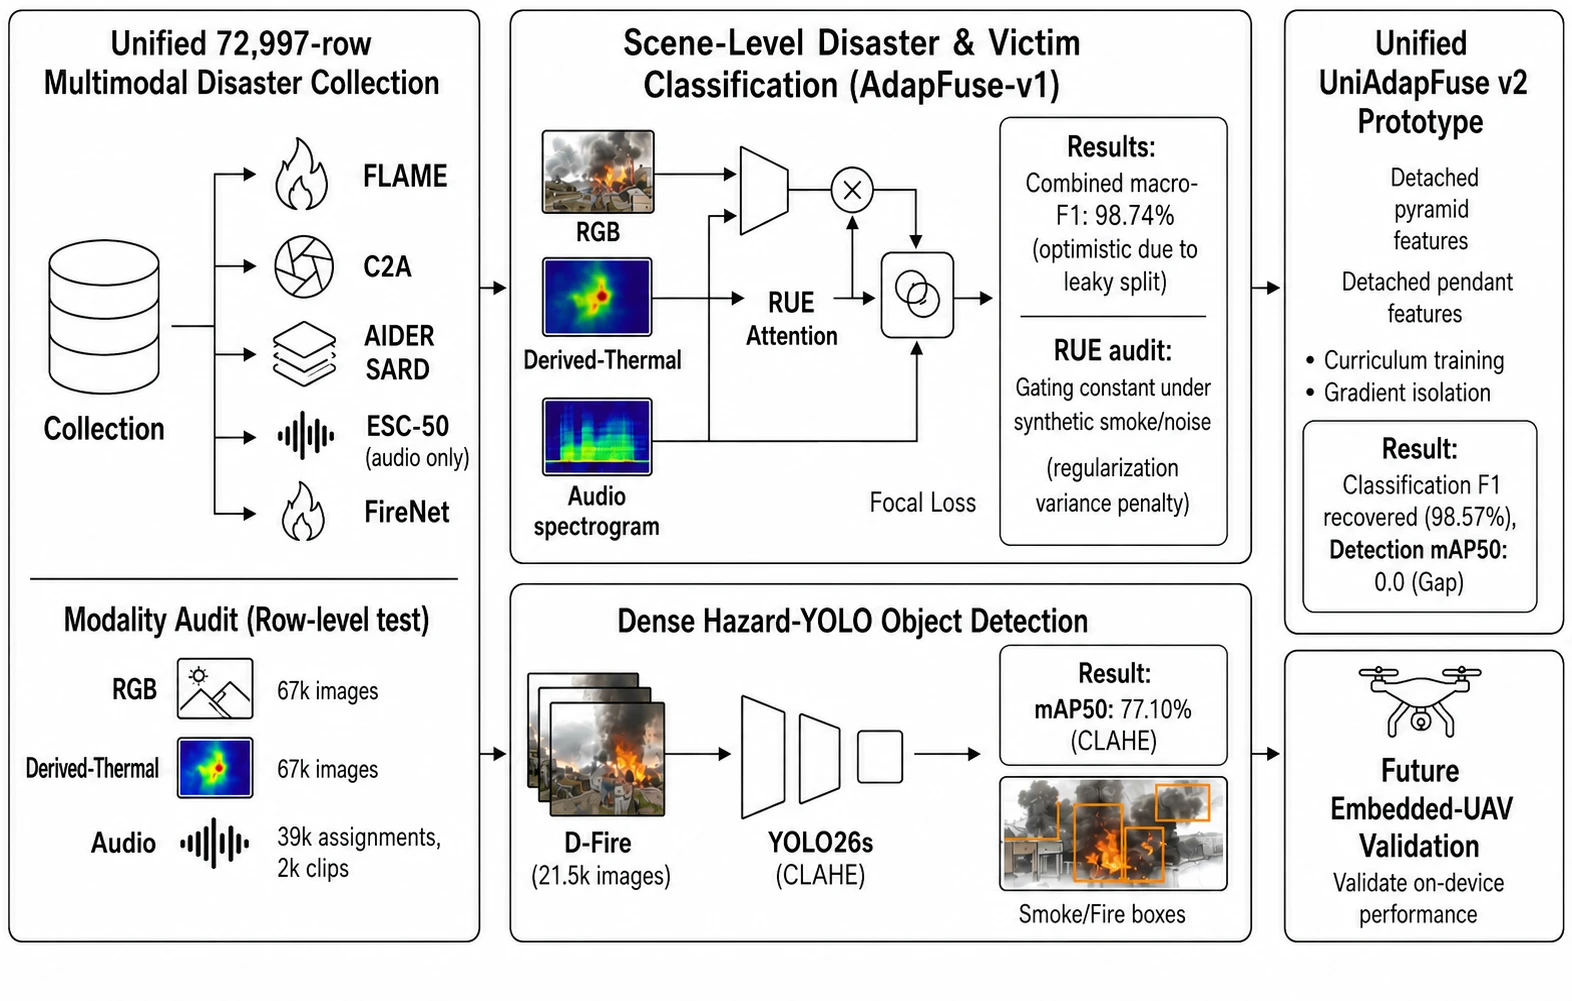
\includegraphics[width=\textwidth]{images/generated/1.png}
    \caption{Evidence-grounded overview of the project. The 72{,}997-row heterogeneous multimodal collection supports scene-level disaster and victim-presence classification, while the independent 21{,}527-image D-Fire benchmark supports smoke/fire bounding-box detection. Solid boxes report measured results; dashed boxes mark the UniAdapFuse detection-validation gap and future embedded-UAV deployment.}
    \label{fig:system_architecture}
\end{figure}

\subsection{Phase 1: Dataset Assembly}

A unified 72{,}997-sample dataset was assembled from six public sources covering wildfire, structural collapse, crowd, and victim-presence scenarios:

\begin{itemize}
    \item \textbf{FLAME}~\cite{shamsoshoara2021aerial}: 47{,}992 UAV wildfire RGB frames, the largest source at 65.7\% of the dataset. In our metadata, its thermal entries are RGB-derived pseudo-thermal maps rather than sensor IR.
    \item \textbf{C2A}: 10{,}215 collapse and crowd aerial samples.
    \item \textbf{AIDER}~\cite{kyrkou2019aider}: 6{,}433 multi-class aerial disaster images (wildfire, flood, collapse, traffic).
    \item \textbf{SARD}: 5{,}755 search-and-rescue person-detection frames.
    \item \textbf{ESC-50}~\cite{piczak2015esc}: 2{,}000 environmental sound clips matched to visual samples by disaster label only, not by synchronized capture. A single clip is paired with many images from unrelated scenes, so the audio carries no information about the specific event in each image.
    \item \textbf{FireNet}: 602 fire and non-fire RGB frames.
\end{itemize}

For every RGB source in our metadata, pseudo-thermal maps were generated from the RGB frame; the metadata contains no sensor-IR path. ESC-50 clips were assigned to visual rows by label rather than synchronized capture: 39{,}003 rows reference only 2{,}000 unique audio files. A missing-modality flag tracks unavailable inputs, and training applies 20\% random single-modality dropout. The dataset was split by disaster-label stratification ($n_\text{train}=51{,}097$, $n_\text{val}=10{,}949$, $n_\text{test}=10{,}951$; total 72{,}997 rows). This split is not source-, flight-, or sequence-grouped, so its test metrics are within-collection rather than cross-flight estimates. A capture-group-aware split was therefore rebuilt (50{,}845 / 11{,}055 / 11{,}097 rows across 9{,}267 / 2{,}003 / 2{,}002 disjoint capture groups) and AdapFuse-v1 retrained on it: combined macro-F1 falls from 98.74\% to 89.14\%. That retraining was run without class balancing and with batch size 2, so the drop does not isolate the leakage effect (Section~\ref{sec:grouped_split}).

\textbf{Class balancing:} The raw training split is heavily imbalanced: fire/smoke (46.5\%), clean (41.0\%), collapse/flood (8.5\%), other (4.0\%). Due to a single-GPU resource constraint (NVIDIA RTX 5090, 32\,GB VRAM), a two-stage oversampling procedure was applied to generate a \textit{Stratified Balanced Training} configuration. Stage 1 oversamples each disaster class to the majority-class count via replacement sampling, marking synthetic duplicates with a synthetic-row indicator for stronger augmentation. Stage 2 oversamples the victim-positive class to achieve 50/50 victim balance while preserving disaster balance. The resulting full-balanced split (98{,}556 samples) is then halved with source-stratified sampling, which keeps all six dataset sources represented, yielding the final training split of 49{,}276 samples (exactly 12{,}319 per disaster class; 48.1\% synthetic rows). An equivalent procedure produces the validation split (10{,}516 stratified balanced samples). The held-out test set (10{,}951 samples) is \emph{never} resampled and retains the natural class distribution of the collection.

\subsection{Phase 2: Architecture Design}

Six core fusion designs along with architectural variants were implemented and compared under identical training conditions:

\textbf{Unimodal baselines:} Design A1 (RGB-only MobileNetV3-Small), A2 (Thermal-only ResNet-18), and A3 (Audio-only 2D-CNN on mel-spectrograms) established per-modality performance bounds.

\textbf{Early Fusion (Design B):} A five-channel ResNet-18 receiving concatenated RGB, pseudo-thermal, and mel-spectrogram projections in the spatial domain.

\textbf{Late Fusion (Design C):} Three independent backbones producing softmax predictions fused by a learned linear combiner.

\textbf{Intermediate Fixed Fusion (Design D):} Backbone features projected to a shared 192-dim space and concatenated before a shared classification head, with no modality weighting.

\textbf{AdapFuse-v1 (Design E), proposed:} Three backbones (MobileNetV3-Small for RGB, ResNet-18 for thermal, 2D-CNN for audio) plus:
\begin{itemize}
    \item \textit{Reliability and Uncertainty Estimator (RUE):} An MLP reading 16-dim quality tokens and feature statistics per modality, producing scalar gates $r_i \in [0,1]$. In the reported training runs these gates are learned through task loss and a cross-modality variance regularizer, not explicit degradation labels.
    \item \textit{Cross-modal attention:} 4-head attention over reliability-weighted projected tokens stacked across all three modalities.
    \item \textit{NuisanceAwareHead:} The model defines disaster, victim-presence, and five-category nuisance logits. The current trainer supplies no nuisance ground truth, so only the disaster and victim branches are supervised in the reported checkpoints; nuisance-aware learning remains an architectural provision rather than an evaluated contribution.
\end{itemize}

\textbf{AdapFuse-v2 (Design F), knowledge-distilled student:} AdapFuse-v1 architecture with projection dimension reduced to 96 (half of the teacher's 192), trained with logit distillation (temperature $T=4.0$) and intermediate feature distillation ($\lambda=0.5$) from the Design E teacher.

\subsection{Phase 3: Training and Evaluation}

All twenty-six multimodal classification models (spanning core fusion designs, visual/acoustic backbone variants, architectural augmentations, two-sensor subsets, unified multi-task architectures, and isolated component ablations) were trained with AdamW (lr = $10^{-3}$, weight decay $10^{-4}$), cosine learning-rate decay with 5-epoch linear warmup, batch size 16 (reduced to 8 for EfficientNet-B0 backbone experiments due to larger feature dimensions), up to 50 epochs with early stopping (patience = 15), and automatic mixed precision (AMP). All row-level models use the Stratified Balanced Training Configuration (49{,}276 samples, exact 25\% per class); the grouped-split retraining (Section~\ref{sec:grouped_split}) is a separate run without class balancing. The implemented objective supports optional nuisance and degradation supervision, but our trainer passes both targets as \texttt{None}. The active base objective is therefore focal task loss plus reliability variance regularization:

\begin{equation}
    \mathcal{L} = w_d\,\text{FL}_{\text{disaster}} + w_v\,\text{FL}_{\text{victim}} + \lambda_r\,[-\operatorname{Var}(\mathbf{r})]
\end{equation}

The configuration files set \texttt{corruption\_prob=0.3}, but the base data-loader construction does not provide a \texttt{corruption\_type}; the explicit smoke, blur, low-light, drift, and audio-noise transforms are therefore not activated in the reported base training run. They are invoked only in the separate synthetic stress-test scripts. Evaluation on the held-out row-level split ($n=10{,}951$) uses macro-F1 for disaster and victim-presence classification. Knowledge distillation for Design F adds logit and feature losses on top of the task losses.

\section{Scopes and Challenges}

\textbf{In Scope:}
\begin{itemize}
    \item Multi-disaster detection (wildfire, structural collapse, crowd) and victim presence detection from UAV-sourced RGB imagery, RGB-derived pseudo-thermal maps, and label-matched acoustic clips~\cite{erdelj2017help}.
    \item Systematic comparison of six fusion architectures from unimodal baselines to adaptive attention-based fusion.
    \item Single-component comparison runs for the one-step GRU, cross-modal attention, learned quality features, auxiliary nuisance branch, and RUE gating.
    \item Investigation of multi-task negative transfer via phased curriculum training and stop-gradient feature isolation.
    \item Knowledge distillation for edge-deployment model compression~\cite{hinton2015distilling}.
    \item An implemented nuisance-class branch, with supervised nuisance learning left for future labeled experiments.
    \item Environmental corruption stress testing across five severity levels, and missing-modality checks through two-sensor subsets and simulated sensor dropout.
\end{itemize}

\textbf{Out of Scope:} Physical in-flight edge deployment on an active UAV airframe with live payload actuation, long-term post-disaster reconstruction planning, and autonomous UAV aerodynamic path planning. These are identified as priority future directions in Chapter~6.

\textbf{Key Challenges Encountered:}
The audio modality presented the most significant practical challenge: ESC-50 clips are general environmental sounds paired by label rather than captured synchronously with the same disaster scene. The audio-only baseline (Design A3) achieved only 38.2\% disaster F1, and the AdapFuse-v1 checkpoint assigns audio a near-zero gate, showing that this constructed channel contributes little. Every populated thermal path points to an RGB-derived pseudo-thermal map, including FLAME and C2A; no sensor-IR frames are present in our metadata. The high prevalence of FLAME creates a visually dominant source, and the row-level split proved to be a substantial explanation for the narrow, near-ceiling performance range: retraining under capture-group-aware splitting scores 9.60 percentage points lower in combined macro-F1, although that retraining also differed in class balancing and batch size. Decomposing those grouped predictions by source exposes a second problem: source identity and label are confounded in the assembled corpus. Victim presence is fully determined by the source dataset in the grouped test set, and several sources contain a single disaster class, so aggregate scores cannot distinguish hazard or person recognition from dataset recognition.
